\documentclass[twocolumn,10pt]{article}

\usepackage[utf8]{inputenc}
\usepackage{amsmath}
\usepackage{amssymb}
\usepackage{booktabs}
\usepackage{microtype}
\usepackage{geometry}
\usepackage{longtable}
\usepackage{graphicx}
\usepackage{pdflscape}
\usepackage{cuted}
\usepackage{verbatim}
\usepackage{float}
\usepackage{caption}
\usepackage{hyperref}

\graphicspath{{figures/}{docs/assets/publishings/figures/}}

\DeclareMathOperator{\sgn}{sgn}

\geometry{a4paper, margin=0.75in}

\title{\textbf{An Analytical Framework for Multi-Variable Non-Linear Damage Superposition in Bounded Discrete Tactical Environments}}
\author{\textbf{BotAn} \\ \small Brown Dust II Tactical Compendium}
\date{\today}

\begin{document}
\raggedbottom

\maketitle

\begin{abstract}
Predicting discrete state-vector outputs in complex tactical computational environments remains an analytical challenge when underlying source code is obfuscated. This paper presents a phenomenological framework that maps the conditional mechanics of the Brown Dust II engine into a unified, declarative formulation. Rather than relying on fragmented imperative conditional branching, a declarative algebraic formulation is constructed by projecting discrete mechanics onto continuous vector spaces and binary archetype coupling operators. By representing elemental attributes as orthogonal property vectors and mapping status modifiers via multidimensional linear transformations, a mathematically rigorous alternative to traditional algorithmic scripting is provided. The resulting architecture establishes a verifiable foundation for automated team optimization, designed to be empirically falsifiable across live server environments.
\end{abstract}

\section{Introduction}
In discrete tactical simulation environments, the determination of state transitions—specifically, the calculation of kinetic and ethereal energy transfer between opposing nodes—is a critical computational process. Modern turn-based architectures have evolved past elementary linear scaling systems, introducing multi-layered, interdependent modifier pools. While these complex mechanics enrich the strategic depth of the environment, they frequently introduce severe optimization challenges for system analysis.

Within the specific framework of the Brown Dust II tactical engine, automated data routing and character configuration require a precise understanding of how discrete attributes scale under active status modifiers. In practical execution, players and developers alike encounter a high-dimensional combinatorial optimization problem when configuring team sequencing matrices. Because the underlying source code of the execution engine remains proprietary and obfuscated, the precise topological structure of these interactions cannot be verified through direct code inspection.

This systemic lack of transparency presents a distinct analytical hurdle. When multiple status-altering modifiers—such as offensive amplifications (e.g., Attack or Magic Attack pooling), temporal damage vectors (Chains), and structural vulnerabilities—interact simultaneously, predicting the exact output state becomes non-trivial. Compounding this challenge is the presence of hard operational boundary limits, such as saturation caps applied to entity vitality metrics, which inject non-linear constraints into otherwise predictable algebraic equations.

To resolve these ambiguities, this study adopts a black-box phenomenological approach to reverse-engineer and formalize the global damage system. By conducting systematic, isolated live-server experiments, individual systemic rules are identified, evaluated, and translated from sequential control-flow constraints into a unified mathematical syntax. It is demonstrated that apparent algorithmic discrepancies—such as the transition between additive pooling and multiplicative compounding—can be elegantly modeled using linear algebra and orthogonal basis vector operations.

The primary contributions of this paper are threefold:
\begin{enumerate}
  \item A modular, bottom-up mathematical derivation of individual modifier behaviors constructed entirely from empirical observation.
  \item The formulation of a unified master equation that encodes conditional runtime branching into declarative algebraic coupling operators.
  \item Computational verification proving that the proposed declarative model achieves absolute predictive convergence with live system executions.
\end{enumerate}

The structural composition of the remainder of this document is organized as follows. Section~\ref{sec:derivation} details the phase-by-phase axiomatic construction of individual scaling components and establishes the mathematical rationale behind additive buff stacking constraints. Section~\ref{sec:master_formula} synthesizes these isolated components into a single, comprehensive master equation. Section~\ref{sec:validation} establishes the empirical foundation required for algorithmic team matrix optimization. Finally, Section~\ref{sec:conclusion} discusses the architectural implications of the decoupled pipeline, evaluates practical optimization boundaries, and outlines future empirical objectives.

% =========================================================================
% SECTION II: SYSTEM MODELING AND CORE VECTOR MECHANICS
% =========================================================================
\clearpage
\section{System Modeling and Core Vector Mechanics}

\label{sec:derivation}

To construct a verifiable mathematical model of the calculation pipeline, the game's underlying execution engine is analyzed by gradually introducing systemic complexities. This progressive approach ensures that the mathematical framework remains tightly aligned with observable live-server behavior.

Throughout this framework, while in-game interfaces display status attributes and modifier ratings in percentage syntax (e.g., $+150\%$ Crit Damage or $90\%$ DEF), all mathematical parameters are evaluated in normalized, dimensionless scalar units (where $100\% \equiv 1.0$). Unless explicitly stated otherwise via floor operators ($\lfloor \dots \rfloor$), variables maintain floating-point precision across intermediate pipeline stages.

\subsection{The Elementary Scalar Model}
The most intuitive baseline model assumes a standard physical interaction where a source unit executes an action against a single target tile occupied by a neutral target unit. In this idealized state, devoid of active status modifiers, elemental properties, or defensive mitigation mechanics, the primary baseline damage output ($D_0$) can be expressed as a basic scalar product:
\begin{equation}
D_0 = \text{ATK} \cdot M
\label{eq:scalar_base}
\end{equation}
where $\text{ATK}$ represents the flat physical attack attribute of the source unit, and $M$ denotes the scaling multiplier dictated by the active skill. While Equation~\ref{eq:scalar_base} successfully accounts for elementary, single-variable physical interactions, it quickly fails when confronted with more sophisticated unit skill sets.

Crucially, this framework isolates the atomic execution kernel that computes outgoing damage dealt to a target node. Downstream runtime events — specifically target vitality subtraction and secondary barrier depletion cascades are treated as external consumer processes and remain outside the scope of this kernel.

\subsection{The Attribute Dependency Conflict}
Empirical testing across diverse unit skill sets reveals that the calculation engine does not utilize a single, uniform attribute for output evaluations. Instead, independent character and costume skill designs shift their scaling dependencies dynamically across entirely distinct statistical pools:
\begin{enumerate}
    \item \textbf{Magical Payloads:} Certain skill sets completely swap physical parameters for a magical alternative, forcing the baseline calculation to rely on $\text{MATK} \cdot M$
    \item \textbf{Vitality Scaling:} Advanced tank-type units leverage alternative skill designs that bypass offensive statistics entirely, generating an output value scaled by the source unit's own maximum health points ($\text{HP} \cdot M$).
    \item \textbf{Simultaneous Multi-Attribute Scaling:} The most critical analytical conflict occurs with hybrid skill sets that track multiple independent metrics simultaneously. For example, specific protective mechanics compute an execution value based on the concurrent summation of both the source unit's current Health Points and their active protective layers (Energy Guard, $\text{EG}$) on a localized target tile.
\end{enumerate}
Attempting to model these fluid, multi-variable dependencies using standard scalar mathematics would require a disjointed set of nested conditional control statements. To maintain a clean, declarative mathematical framework that handles single-attribute and multi-attribute calculations uniformly, a structural shift from scalar spaces to vector spaces is required.

\subsection{Vector Space Formalization and Operational Constraints}
\label{sec:vector_space}
To elegantly resolve the multi-attribute dependencies identified above, alongside interactive mechanics that scale dynamically based on target unit metrics, the interaction state is compiled into a unified, eight-dimensional column vector, designated as the Source-Target Stat Vector, $\vec{v} \in \mathbb{R}^8$:
\begin{equation}
\vec{v} = \begin{pmatrix} 
\text{ATK}_{\text{src}} \\ 
\text{MATK}_{\text{src}} \\ 
\text{HP}_{\text{src}}^{\text{MAX}} \\
\text{EG}_{\text{src}} \\ 
\text{ATK}_{\text{tgt}} \\ 
\text{MATK}_{\text{tgt}} \\ 
\text{HP}_{\text{tgt}}^{\text{MAX}} \\
\text{HP}_{\text{tgt}}^{\text{Current}} 
\end{pmatrix}
\end{equation}
This vertical coordinate space maps the primary offensive parameters alongside vitality pools for both the source entity and the target entity simultaneously.

At the database level, the system enforces strict structural boundaries on the elements of $\vec{v}$ based on the character templates assigned to the respective units. Because any individual unit asset is hardcoded to belong exclusively to either a physical or a magical archetype, the active offensive parameters within the vector space must satisfy a pair of decoupled zero-product boundary conditions:
\begin{equation}
v_1 \cdot v_2 = 0 \quad (\text{ATK}_{\text{src}} \cdot \text{MATK}_{\text{src}} = 0)
\label{eq:exclusivity_src}
\end{equation}
\begin{equation}
v_5 \cdot v_6 = 0 \quad (\text{ATK}_{\text{tgt}} \cdot \text{MATK}_{\text{tgt}} = 0)
\label{eq:exclusivity_tgt}
\end{equation}
These conditions ensure that if a unit configuration yields active physical parameters ($\text{ATK} \neq 0$), its corresponding magical component is fundamentally driven to zero ($\text{MATK} = 0$), and vice versa. Vitality metrics face no such structural constraints and exist simultaneously across all active unit entities.

To interface with this combined attribute snapshot, the executing skill set maps its specific scaling coefficients into a matching eight-dimensional column vector, designated as the Skill Scaling Vector, $\vec{m} \in \mathbb{R}^8$
\begin{equation}
\vec{m} = \begin{pmatrix} m_1 & m_2 & m_3 & m_4 & m_5 & m_6 & m_7 & m_8 \end{pmatrix}^{\top}
\end{equation}
All individual scaling coefficients within the Skill Scaling Vector are bound by a strict non-negativity constraint, such that $m_i \ge 0$ for all element index positions $i \in \{1, \dots, 8\}$. This structural floor ensures that a baseline skillset execution can only generate constructive or neutral payload components, mathematically isolating all reductive transformations to the external debuff pools and adversarial mitigation layers evaluated later in the pipeline.

To calculate the active interaction payload components across all eight statistical channels simultaneously, we can apply an element-wise Hadamard product ($\circ$) between the two column vectors, creating an intermediate column Execution Vector, $\vec{e} \in \mathbb{R}^8$:
\begin{equation}
\vec{e} = \vec{v} \circ \vec{m}
\label{eq:hadamard_exec}
\end{equation}
where each individual element is evaluated via scalar multiplication as $e_i = v_i \cdot m_i$. Utilizing the element-wise mapping of the Hadamard product is mathematically mandatory for this system configuration; it ensures that independent statistical properties remain completely isolated before final summation. This architectural choice allows subsequent environmental modifier fields to be mapped onto the system as independent vector operations.

The final, unmitigated base damage output ($D_0$) for the targeted tile is then extracted by evaluating the sum of the resulting execution elements:
\begin{equation}
D_0 = \sum_{i=1}^{8} e_i = \sum_{i=1}^{8} v_i \cdot m_i
\label{eq:hadamard_sum}
\end{equation}

This formulation successfully unifies the underlying system mechanics under a single declarative rule. For a standard physical interaction, Equations~\ref{eq:exclusivity_src} and \ref{eq:exclusivity_tgt} force the magical elements of the active unit profiles to zero. Consequently, the intermediate Execution Vector $\vec{e}$ evaluates to an axis-aligned state containing only the active physical payload components, rendering the final summation in Equation~\ref{eq:hadamard_sum} mathematically equivalent to an elementary scalar model. For hybrid or target-interactive skill sets, the Hadamard framework natively preserves the distinct parallel channels for vitality metrics and target scaling values, mapping out their simultaneous contributions before final aggregation without requiring fragmented conditional code branches.

\subsection{Base Attribute Construction and Level Dependencies}
The individual elements compiled within the Source-Target Stat Vector $\vec{v}$ are not primitive, static constants pulled directly from character sheets. Instead, a structural division exists between persistent, macro-progression attributes controlled by the source entity, transient combat barrier metrics, and external values mirrored from the target state node. 

For the native, persistent source attribute channels $v_i$ where $i \in \{1, 2, 3\}$ (corresponding explicitly to $\text{ATK}_{\text{src}}$, $\text{MATK}_{\text{src}}$, and $\text{HP}_{\text{src}}^{\text{max}}$ respectively), each element represents the dynamic terminal output of a multi-layered Attribute Aggregation Phase. Live-server empirical research reveals that the engine evaluates a strict hierarchical sequence of level-scaling, flat additions, and global percentage modifiers to construct these final pre-combat stat parameters before grid deployment.

To formalize this persistent pipeline, let $S_{\text{base}}$ represent the initial, native baseline value of a given source attribute channel $i$. The level-dependent growth curve is driven by a linear scaling coefficient, $\alpha_i$ (for $ i \in \{1,2,3\}$), determined explicitly by the category of the target attribute:
\begin{equation}
\alpha_i = 
\begin{cases} 
0.1 & \text{if } i = 1 \text{ or } 2 \quad (\text{ATK}_{\text{src}} \text{ or } \text{MATK}_{\text{src}}) \\ 
0.2 & \text{if } i = 3 \quad (\text{HP}_{\text{src}}^{\text{max}}) 
\end{cases}
\label{eq:growth_coeff}
\end{equation}
Crucially, while Equation~\ref{eq:growth_coeff} evaluates a non-zero linear progression rate for both offensive channels, the structural boundary constraint established in Equation~\ref{eq:exclusivity_src} dictates that the vacant archetype channel initiates with a baseline property value of $S_{\text{base}} = 0$, rendering its concurrent level aggregation trivially zero.

By utilizing this coefficient alongside the unit's current level ($L$), the absolute flat component accumulation value ($v_{i,\text{flat}}$) aggregates native growth concurrently with flat numerical additions from gear configurations, active or permanent bond systems, and awakening milestones:
\begin{equation}
\begin{split}
v_{i,\text{flat}} = {} & \left\lfloor S_{\text{base}}\left(1 + \alpha_i \cdot L \right)\right\rfloor \\
& + A_{\text{gear\_flat}} + A_{\text{bond\_flat}} + A_{\text{awake\_flat}}
\end{split}
\label{eq:flat_stat_construction}
\end{equation}

At the gear aggregation layer, non-archetype offensive affixes are systematically masked: if a unit's native archetype is magical ($S_{\text{base}} = 0$ for $i=1$), all flat and percentage physical equipment rolls are zeroed by the engine ($A_{\text{gear\_flat}, 1} = 0$), and vice versa. This operational masking preserves the zero-product condition ($v_1 \cdot v_2 = 0$) across persistent macro-progression states.

Once $v_{i,\text{flat}}$ is established, the engine evaluates a unified multiplicative layer containing all passive, permanent, and equipment-based percentage scaling pools to yield the compound coefficient channel, $v_{i,\text{field}}$:
\begin{equation}
\begin{split}
v_{i,\text{field}} = {} & 1 + \omega_{\text{collection}} + \omega_{\text{gear}} \\
& + \omega_{\text{awakening}} + \omega_{\text{bond\_temp}} + \omega_{\text{bond\_perm}}
\end{split}
\label{eq:field_stat_construction}
\end{equation}
where each $\omega$ term represents the fractional value of its respective percentage bonus pool. The terminal active value loaded into these persistent vector coordinates is subsequently computed as the direct product of these two distinct structural phases:
\begin{equation}
v_i = \left\lfloor v_{i,\text{flat}} \cdot v_{i,\text{field}} \right\rfloor \quad \text{for } i \in \{1, 2, 3\} 
\label{eq:final_vector_element}
\end{equation}

In contrast to the persistent attribute pipeline, the protective Energy Guard layer channel $v_4$ ($\text{EG}_{\text{src}}$) represents a highly volatile, dynamic instance state rather than an internal progression attribute. Because defensive Guard parameters are generated at runtime through diverse external skill variables and non-native scaling references, $v_4$ fundamentally bypasses Equations~\ref{eq:growth_coeff} through \ref{eq:final_vector_element}. Instead, the engine isolates this slot from the macro-progression accumulation layer, populating $v_4$ directly via a real-time snapshot of the absolute active Energy Guard shielding remaining on the source node's grid matrix location at the exact execution frame.

This synthesis successfully concludes the initialization and consolidation of the active attribute parameters. By fully encapsulating all character growth, equipment additions, and passive account progressions directly within the core source coordinates $v_1$ through $v_4$, the system establishes a stable, fully aggregated dataset ready to be processed through the localized skillset execution layers, while elements $v_5$ through $v_8$ are concurrently mirrored from the corresponding target unit's independent aggregation layer at the moment of runtime execution.

\subsection{Operational Bounds and Intermediate Precision}
To enforce foundational system invariants, damage transactions are subject to a strict constructive positivity floor, guaranteeing $D \ge 1$. In the evaluation hierarchy, discrete attribute channels (such as $\text{ATK}$, $\text{MATK}$, and $\text{HP}$) undergo integer truncation at macro-progression and active-state aggregation boundaries (Eqs.~\ref{eq:flat_stat_construction}, \ref{eq:final_vector_element}, and \ref{eq:v_active}), and the resulting base payload $M_{\text{base}}$ is floored prior to combat multiplier resolution (Eq.~\ref{eq:base_modulated_damage}). Conversely, percentage-denominated multiplier channels (Critical, Property, Combo Chain, Vulnerability, and Reductive Barrier) preserve full floating-point precision throughout calculation, with terminal integer flooring applied strictly at final damage synthesis (Section~\ref{sec:terminal_damage_synthesis}).
\subsection{Skill Scaling Vector Construction}
\subsubsection{Skills}
Skill scaling parameters are derived from the skill's inherent design and are influenced by Costume upgrade level, Potential Liberation nodes, and Burst mechanics, alongside dynamic conditional dependencies on target or source unit states. Each active Skill Scaling Vector element $m_i$ evaluates as:
\begin{equation}
\label{eq:skill_scaling_element}
m_i = m_i^{(\text{costume})}[c] + \sum_j \Delta m_{i,j}^{(\text{liberation})} + \sum_j \Delta m_{i,j}^{(\text{burst})}
\end{equation}
where $c \in \{0, \dots, 5\}$ denotes the discrete costume upgrade tier ($+0$ through $+5$). 

For skillsets that exhibit spatial or state dependencies, the scalar elements $m_i$ modulate dynamically via localized indicator flags (e.g., discrete main-target terms $m_i + \Delta m \cdot \delta_{\text{MT}}$ where $\delta_{\text{MT}} \in \{0, 1\}$, or cumulative debuff multipliers $m_i + \Delta m \cdot N_{\text{debuff}}$).
\subsubsection{Basic Attacks}
Basic Attacks can be represented as a special case of the general skill scaling framework, where the scaling coefficients are determined by the character's base attack pattern and are not influenced by external factors such as costume upgrades or potential liberations. For Basic Attacks, the Skill Scaling Vector Elements $m_1$ and $m_2$ (corresponding to physical and magical attack scaling respectively) can be both set to 1 due to constraint on the Source-Target Stat Vector, while all other elements are set to 0, resulting in the following Skill Scaling Vector:
\begin{equation}
  \vec{m}_{\text{BA}} = \begin{pmatrix} 
  1 \\ 
  1 \\ 
  0 \\ 
  0 \\ 
  0 \\ 
  0 \\ 
  0 \\
  0
  \end{pmatrix}
\end{equation}

\subsubsection{Knockbacks}
Knockback is another special case of the general skill scaling framework, where the damage is always set to 1 (do not confuse with collision damage caused by the knockback itself). Since the damage output is fixed, the Skill Scaling Vector for Knockbacks can be represented as a null vector:
\begin{equation}
  \vec{m}_{\text{KB}} = \vec{0}
\end{equation}
In other words, all elements of the Skill Scaling Vector for Knockbacks are set to 0, indicating that the damage output does not scale with any of the source or target attributes.

\subsubsection{Collision Damage}
While primary combat modeling addresses direct source-target skillset interactions, collision damage resulting from knockback displacement can be incorporated as a secondary pairwise interaction. In this secondary transfer, the displaced unit acts as the intermediate source and the impacted entity serves as the target, scaling from the source unit's vitality pool ($m_3$).

For the collision damage inherited from the simple knockback, $m_3$ is set to a fixed value of 0.25, while all other elements are set to 0, resulting in the following Skill Scaling Vector:
\begin{equation}
  \vec{m}_{\text{CD}} = \begin{pmatrix} 
  0 \\ 
  0 \\ 
  0.25 \\ 
  0 \\ 
  0 \\ 
  0 \\ 
  0 \\
  0
  \end{pmatrix}
\end{equation}
However, if the knockback is caused by a skill that has different scaling coefficient for the knocked back unit's HP, then $m_3$ will be set to that scaling coefficient instead of 0.25.

\subsection{High-End Ceiling to Source-Target Stat Vector}

To avoid unexpected behavior during calculations, as well to prevent unwanted scaling, restraints to the values of Source-Target Stat Vector are applied by in-game engine.

These can be expressed via Ceiling Vector $\vec{C}$:

\begin{equation}
  \vec{C} = \begin{pmatrix} 
  10^5\\ 
  10^5 \\ 
  5 \times 10^4 \\
  \infty \\ 
  10^5\\ 
  10^5 \\ 
  5 \times 10^4 \\
  5 \times 10^4
  \end{pmatrix}
\end{equation}

To enforce these operational boundaries, the component-wise minimum between each coordinate $v_i$ and its respective ceiling $C_i$ is evaluated. In an unmodulated baseline environment, this yields the bounded payload:
\begin{equation}
\label{eq:base_unmodulated}
M_{\text{base}, 0} = \left\lfloor \min_\circ \left(\vec{C}, \vec{v} \right)^\top \vec{m} \right\rfloor
\end{equation}
Under active combat modulation, this ceiling operation is applied directly to the dynamic active stat vector $\vec{v}_{\text{active}}$ (Section~\ref{sec:master_formula}, Eq.~\ref{eq:base_modulated_damage}).

The finite threshold defined in $\vec{C}$ for vitality channels ($C_3, C_7, C_8 = 5 \times 10^4$) enforces an internal calculation saturation ceiling across both source and target entities. For target coordinates ($v_7, v_8$), this boundary prevents percentage-based target vitality skills from scaling unbounded against structured raid bosses whose vitality pools routinely exceed $10^8$. Symmetrically, capping the source coordinate ($v_3$) enforces an operational ceiling on offensive vitality-scaling skill sets, preventing high-health tank archetypes from generating unbounded baseline payloads under extreme macro-progression vitality stacking.
\subsection{Dynamic Attribute Modulation and Environmental Pressure}

Various environmental interactions and combat effects dynamically alter the components of the Source-Target Stat Vector, encompassing both positive amplification and negative attenuation across active channels.

The algebraic formulation established in this section applies analogously to all subsequent multiplier layers and will be referenced uniformly throughout the remainder of this framework.

\subsubsection{Positive Dynamic Attribute Modulation}

Positive dynamic attribute modulations — designated as Stat Reinforcements (Buffs) — amplify specific attribute channels additively. Applying these active enhancements transforms the baseline state vector $\vec{v}$ into the modulated expression:

\begin{equation}
\label{eq:pos_dyn_attr_mod}
  \vec{v} \circ \left(\vec{1} + \sum_{j}{\vec{b}_{j}^{\text{(off)}}}\right)
\end{equation}

From here on, summation operators of the form $\sum_j \vec{\mathbf{b}}_j^{(\text{type})}$ implicitly iterate over all active, non-zero modifier instances within the designated category.

Given form represents Attribute Modulations for Source-Target Stat Vector in a space $\mathbb{R}^8$, allowing constructive modifiers to scale respective source and target channels in parallel while preserving the underlying coordinate orthogonality of the system.

\subsubsection{Negative Dynamic Attribute Modulation}

Unlike positive modulations, negative dynamic attribute modulations (debuffs) decrease specific attribute channels. They operate additively and contribute directly alongside positive reinforcements, transforming Expression~\ref{eq:pos_dyn_attr_mod} into:
\begin{equation}
  \label{eq:neg_dyn_attr_mod}
  \vec{v} \circ \max_\circ \left(\vec{0}, \left(\vec{1} + \sum_{j}{\vec{b}_{j}^{\text{(off)}}} - \sum_{j}{\vec{d}_{j}^{\text{(off)}}} \right) \right)
\end{equation}

Here, the scalar components of each modifier vector are defined as non-negative ($b_{j,i} \ge 0$, $d_{j,i} \ge 0$ for all channels $i \in \{1, \dots, 8\}$). While negative modulations could theoretically be modeled as a special case of generalized signed vectors, isolating debuffs into an explicitly subtracted non-negative pool preserves algebraic clarity across subsequent pipeline transformations.

Enforcing a strict lower bound at zero is empirically corroborated by live-server testing: when cumulative debuffs exceed total positive amplifications ($\sum_j \vec{b}_j^{(\text{off})} - \sum_j \vec{d}_j^{(\text{off})} \le -\vec{1}$), the active attribute parameters clamp strictly at zero rather than evaluating to negative values.

\subsubsection{Environmental Pressure}

Environmental Pressure ($P$) acts as an external attenuation scalar applied strictly against Stat Reinforcement modifier pools (specifically ATK, MATK, Crit Rate, Crit Damage, Property, and DEF/MRES). Multiplier channels governed by kinetic combo chains, outgoing damage augmentations, and target incoming vulnerability debuffs operate independently of Pressure. Furthermore, vitality and shield coordinates ($v_3, v_4, v_7, v_8$) do not receive active combat stat reinforcements, rendering their respective buff vectors identically zero ($\vec{b}_j = \vec{0}$).

\begin{equation}
  P = 1 - \min \left( 1, \sum_{j}{\text{Pr}_j} \right)
\end{equation}

This implies that multiple Pressure effects add linearly, with 100\% or more Pressure negating any positive modulation. Applying this attenuation factor directly to the positive reinforcement pool in Expression~\ref{eq:neg_dyn_attr_mod} yields:
\begin{equation}
  \label{eq:dyn_attr_mod}
  \vec{v} \circ \max_\circ \left(\vec{0}, \left(\vec{1} + \sum_{j}{\vec{b}_{j}^{\text{(off)}}} \cdot P - \sum_{j}{\vec{d}_{j}^{\text{(off)}}} \right) \right)
\end{equation}

For simplicity, the Modifier Transformation Operator $\hat{\mathcal{T}}$ is defined as:

\begin{equation}
 \hat{\mathcal{T}} (\{\vec{b}_j\}, \{\vec{d}_j\}, P) = \sum_{j}{\vec{b}_{j}} \cdot P - \sum_{j}{\vec{d}_{j}}
\end{equation}

and for scalar representation:

\begin{equation}
 \hat{\mathcal{T}} (\{b_j\}, \{d_j\}, P) = \sum_{j}{b_{j}} \cdot P - \sum_{j}{d_{j}}
\end{equation}

This form simplifies the Expression~\ref{eq:dyn_attr_mod}, allowing to finalize the multiplier, tied to the Source-Target Stat Vector, in the following expression:

\begin{equation}
\label{eq:v_active}
  \vec{v}_{\text{active}} = \left\lfloor \vec{v} \circ \max_\circ \left( \vec{0}, \; \vec{1} + \hat{\mathcal{T}}\big(\{\vec{b}_j^{(\text{off})}\}, \{\vec{d}_j^{(\text{off})}\}, P\big) \right) \right\rfloor
\end{equation}

\begin{equation}
\label{eq:base_modulated_damage}
  M_{\text{base}} = \left\lfloor \min_\circ \left( \vec{C}, \; \vec{v}_{\text{active}} \right)^\top \vec{m} \right\rfloor
\end{equation}

The floor operator $\lfloor \dots \rfloor$ reflects the engine's truncation of the unmitigated baseline damage payload to a discrete integer prior to evaluating external combat multiplier brackets.

\subsection{Adversarial Mitigation Mechanics}

Damage mitigation in the execution engine operates through two distinct layers: kinetic resistance (Physical Defense, $\text{DEF}$, and Magic Resistance, $\text{MRES}$) and absorption layers (Barriers). This section formalizes the kinetic resistance channel, while Barrier cascades are treated in Section~\ref{sec:barriers}.

Similar to offensive parameters, baseline defensive attributes represent persistent pre-combat accumulations:
\begin{equation}
\text{DEF}_{\text{tgt}} = k_{\text{collection}} + k_{\text{gear}} + k_{\text{awakening}} + k_{\text{bond}}
\end{equation}
with $\text{MRES}_{\text{tgt}}$ constructed analogously across equivalent progression pools.

Dynamic combat reinforcements and shred debuffs scale these attributes additively via the transformation operator $\hat{\mathcal{T}}$. Because the source exclusivity boundary condition enforces $v_1 \cdot v_2 = 0$ (Equation~\ref{eq:exclusivity_src}) and $\vec{v} \ge 0$, the target's active effective resistance metric $R_{\text{tgt}}$ is projected strictly along the attacker's native kinetic domain:
\begin{equation}
\label{eq:r_tgt_modulated}
\begin{split}
  R_{\text{tgt}} = {} & \sgn(v_1) \cdot \left[ \text{DEF}_{\text{tgt}} + \hat{\mathcal{T}}\left(\{b^{(\text{def})}_j\}, \{d^{(\text{def})}_j\}, P\right) \right] \\
  & + \sgn(v_2) \; \cdot \\
  &\left[ \text{MRES}_{\text{tgt}} + \hat{\mathcal{T}}\left(\{b^{(\text{mres})}_j\}, \{d^{(\text{mres})}_j\}, P\right) \right]
\end{split}
\end{equation}

This projection guarantees that physical strikes ($v_1 > 0$) are mitigated solely by physical defense channels, while magical strikes ($v_2 > 0$) route exclusively to magic resistance pools.

The discrete signum projections $\sgn(v_1)$ and $\sgn(v_2)$ route adversarial mitigation according to the source entity's persistent archetype classification rather than individual skill scaling dependencies. Under this architecture, alternative scaling skills (such as HP-scaling attacks executed by physical archetype units) route exclusively into physical mitigation pools. It is crucial that the suggested routing using $\textit{sgn}$ function, relies on unmodulated base coordinates, rather than active coordinates $v_{1,\text{active}}, v_{2,\text{active}}$.

Additionally, several operational constraints are enforced. To prevent complete damage nullification, an effective resistance ceiling of $90\%$ is maintained (yielding a minimum multiplier floor of $0.10$). Conversely, resistance cannot drop below $0\%$ (capping the maximum damage yield at $1.0$). Enforcing these boundary limits yields the standard mitigation expression:
\begin{equation}
\label{eq:def_bracket_nodmgtype}
  M_{\text{res}} = \min \Big( 1, \; \max \left( 0.1, \; 1 - R_{\text{tgt}} \right) \Big)
\end{equation}

\subsubsection{Damage Type Variations and Mitigation Penetration}
\label{sec:damage_type_introduction}
Certain kinetic payloads bypass target mitigation layers entirely. Specifically, interactions classified as \textit{Fixed}, \textit{Consumed}, or \textit{Pure} damage exhibit complete invariance to adversarial resistance pools ($\text{DEF}$ and $\text{MRES}$).

To capture this behavior declaratively without branching conditional statements, we define the binary Defensive Coupling Factor $\gamma_{\text{def}} \in \{0, 1\}$:
\begin{equation}
  \label{eq:gamma_def}
  \gamma_{\text{def}} = 
  \begin{cases} 
    0 & \text{if } \text{type} \in \{\text{Pure}, \text{Fixed}, \text{Consumed}\} \\ 
    1 & \text{otherwise (Standard Payloads)} 
  \end{cases}
\end{equation}

When evaluating mitigated interactions, $\gamma_{\text{def}} = 1$ preserves the full resistance transformation. Conversely, for penetrating damage archetypes, $\gamma_{\text{def}} = 0$ nullifies the defensive bracket, collapsing the bracket to the unmitigated baseline multiplier of $1.0$.

Coupling $\gamma_{\text{def}}$ into Expression~\ref{eq:def_bracket_nodmgtype} yields the terminal Resistance Multiplier $M_{\text{res}}$:
\begin{equation}
\label{eq:def_bracket_dmgtype}
  M_{\text{res}} = \min \Big( 1, \; \max \left( 0.1, \; 1 - \gamma_{\text{def}} \cdot R_{\text{tgt}} \right) \Big)
\end{equation}

\subsection{Stochastic Energy Scaling}

Stochastic Energy Scaling is introduced via Crit mechanic, that triggers additional damage if conditions are met. In the very basic form, it can be written as

\begin{equation}
\label{eq:crit_multiplier}
  M_{\text{crit}} = 1 + \delta_{\text{crit}} \cdot \text{CDMG}
\end{equation}

Here, $\delta_{\text{crit}}$ is a stochastic trigger indicator responsible for a ``trigger" behavior, and $\text{CDMG}$ (Crit Damage) is responsible for the damage amplification itself.

\subsubsection{Conditional Trigger Modeling}
Since $\delta_{\text{crit}}$ is tied to the source Crit Rate value, it can be rewritten in the following way, ensuring stochastic component is preserved:

\begin{equation}
\label{eq:crit_stochastic}
  \delta_{\text{crit}} = \mathcal{H}(\text{CR} - u), \quad u \sim \mathcal{U}(0, 1)
\end{equation}

where $u$ represents a continuous random variable drawn uniformly from the standard interval $[0, 1)$. This formulation guarantees that a critical hit executes whenever the unit's Critical Rate meets or exceeds the random roll ($\mathcal{H}(x) = 1$ for $x \ge 0$), and evaluates to zero otherwise ($\mathcal{H}(x) = 0$ for $x < 0$).

Expanding the parameters to account for the dynamic attribute modulation gives the following:
\begin{equation}
  \label{eq:crit_rate_nodmgtype}
\delta_{\text{crit}} = \mathcal{H}\left(\max\left(0,v^{\text{(cr)}}+\hat{\mathcal{T}}\left(\{b^{(\text{cr})}_j\}, \{d^{(\text{cr})}_j\}, P\right)\right) - u\right)
\end{equation}

To introduce mechanic that prevents some types of damage to Crit, Coupling Factor $\gamma_{\text{crit}}$ is required:
\begin{equation}
\label{eq:gamma_crit}
  \gamma_{\text{crit}} = 
  \begin{cases} 
    0 & \text{if } \text{type} \in \{\text{Fixed}, \text{Consumed}\} \\ 
    1 & \text{otherwise (Standard Payloads)} 
  \end{cases}
\end{equation}

Additionally, critical hits are guaranteed in specific game modes when an operational threshold of at least 3 chains is established on a target's designated weak tile.

This interaction is formalized by introducing the mode coupling factor $\gamma_{\text{raid}} \in \{0, 1\}$:
\begin{equation}
\label{eq:mode_coupling}
  \gamma_{\text{raid}} = 
  \begin{cases} 
    1 & \text{if mode} \in {\{\text{Fiend Hunter, Guild Raid}\}} \\ 
    0 & \text{otherwise} 
  \end{cases}
\end{equation}

alongside the accumulated weak-tile chain metric $N_{\text{chain}}^{(\text{weak})} \in \mathbb{N}_0$. Crucially, once this threshold is satisfied, the guaranteed critical execution applies globally to all target tiles across the entity, regardless of whether subsequent attacks strike the weak tile directly.

Synthesizing these conditions yields the terminal critical execution indicator $\delta_{\text{crit}}$:
\begin{equation}
  \label{eq:crit_rate_dmgtype}
  \begin{aligned}
\delta_{\text{crit}} &= \gamma_{\text{crit}} \cdot \max \Big(\\
& \mathcal{H}\left(\max\left(0,v^{\text{(cr)}}+\hat{\mathcal{T}}\left(\{b^{(\text{cr})}_j\}, \{d^{(\text{cr})}_j\}, P\right)\right) - u\right), \\
& \gamma_{\text{raid}} \cdot \mathcal{H}\left(N^{(\text{weak})}_{\text{chain}} - 3\right)\Big)
  \end{aligned}
\end{equation}

\subsubsection{Amplitude Amplification and Overflow Conversion}

The damage bonus payload is governed by the source unit's Critical Damage ($\text{CDMG}$) pool. When active attribute enhancements drive the effective Critical Rate beyond the saturation threshold of $100\%$, the engine converts the surplus rate into Critical Damage at a fixed $1:6$ linear ratio ($+600\%$ $\text{CDMG}$ per unit surplus).

Formalizing this excess conversion yields the derived overflow channel, $\Delta \text{CDMG}_{\text{ovf}}$:
\begin{equation}
\label{eq:cdmg_overflow}
\begin{aligned}
  \Delta \text{CDMG}_{\text{ovf}} {}& = 6 \max\Big(0, \; v^{\text{(cr)}}+\hat{\mathcal{T}}\left(\{b^{(\text{cr})}_j\}, \{d^{(\text{cr})}_j\}, P\right) \\
  &- 1\Big)
\end{aligned}
\end{equation}

Integrating this dynamic overflow alongside persistent stats and active modifier pools produces the modulated Critical Damage payload:
\begin{equation}
\label{eq:cdmg_prefinal_1}
\begin{aligned}
  \text{CDMG}_{\text{raw}}  = {}& \max\Big(0, v^{(\text{cdmg})} \\
  &+ \hat{\mathcal{T}}\left( \{b_j^{(\text{cdmg})}\}, \{d_j^{(\text{cdmg})}\}, P \right) \\
  &+ \Delta \text{CDMG}_{\text{ovf}}\Big)
\end{aligned}
\end{equation}

\subsubsection{Amplitude Saturation and Operational Ceiling}

Unlike persistent attribute channels that undergo discrete integer flooring during pre-combat compilation, the Critical Damage ($\text{CDMG}$) payload is evaluated as a continuous floating-point scalar throughout runtime execution. The cumulative payload is bounded strictly by a non-negativity constraint and an upper operational saturation ceiling of $10^4\%$ ($10^2$ in normalized scalar units).

Enforcing these operational boundaries yields the finalized critical amplitude:

\begin{equation}
\label{eq:cdmg_final}
  \text{CDMG} = \min \Big(10^2, \text{CDMG}_{\text{raw}}\Big)
\end{equation}

\subsection{Property Resonance and Elemental Affinity}
\label{sec:elem_matrix}
The directional interaction dynamics between opposing nodes are governed by the Elemental Property System defined over the discrete space $\mathcal{E} = \{\text{Water}, \text{Fire}, \text{Wind}, \text{Light}, \text{Dark}, \text{Neutral}\}$.

Let the active elements of the source and target nodes be represented as standard canonical basis vectors $\mathbf{e}_{\text{src}}, \mathbf{e}_{\text{tgt}} \in \{0, 1\}^6$. The systemic interaction rules are encoded into the Elemental Affinity Matrix $\mathbf{A}_{\text{elem}} \in \mathbb{R}^{6 \times 6}$:

\begin{equation}
\label{eq:elem_matrix}
\mathbf{A}_{\text{elem}} = 
\begin{pmatrix}
0 & 1 & -1 & 0 & 0 & 0 \\
-1 & 0 & 1 & 0 & 0 & 0 \\
1 & -1 & 0 & 0 & 0 & 0 \\
0 & 0 & 0 & 0 & 1 & 0 \\
0 & 0 & 0 & 1 & 0 & 0 \\
0 & 0 & 0 & 0 & 0 & 0
\end{pmatrix}
\end{equation}

The non-zero entries of $\mathbf{A}_{\text{elem}}$ represent a hybrid interaction graph: the cyclic subspace over $\{\text{Water}, \text{Fire}, \text{Wind}\}$ forms a standard antisymmetric tournament ($A_{ij} = -A_{ji}$), whereas the orthogonal $\{\text{Light}, \text{Dark}\}$ subspace represents a symmetric mutual-advantage relation ($A_{45} = A_{54} = 1$). Under Equation~\ref{eq:prop_multiplier}, an interaction where $\omega_{\text{elem}} = +1$ engages offensive property scaling ($\Phi_{\text{off}}$) while assigning a null weight to defensive mitigation ($\max(0, -\omega_{\text{elem}}) = 0$). Consequently, Light and Dark interactions grant mutual offensive amplification without either element suffering defensive property penalty.

Evaluating the bilinear form between the opposing unit vectors yields the scalar Elemental Coupling Factor $\omega_{\text{elem}} \in \{-1, 0, 1\}$:

\begin{equation}
\label{eq:elem_coupling}
  \omega_{\text{elem}} = \mathbf{e}_{\text{src}}^\top \mathbf{A}_{\text{elem}} \, \mathbf{e}_{\text{tgt}}
\end{equation}


Depending on the sign of $\omega_{\text{elem}}$, the engine routes execution to either offensive property amplification ($\Phi_{\text{off}}$) or defensive resistance mitigation ($\Phi_{\text{def}}$):

\begin{equation}
\label{eq:prop_pools}
\begin{aligned}
  \Phi_{\text{off}} &= v_{\text{pr}}^{(\text{off})} + \hat{\mathcal{T}}\left(\{b_j^{(\text{pr\_off})}\}, \{d_j^{(\text{pr\_off})}\}, P\right) \\
  \Phi_{\text{def}} &= v_{\text{pr}}^{(\text{def})} + \hat{\mathcal{T}}\left(\{b_j^{(\text{pr\_def})}\}, \{d_j^{(\text{pr\_def})}\}, P\right)
\end{aligned}
\end{equation}

Synthesizing these modular channels alongside the dedicated Evil Castle modifier yields the consolidated Property Multiplier:

\begin{equation}
\label{eq:prop_multiplier}
\begin{aligned}
  M_{\text{prop}} ={}& \max \Big(0, 1 + \max(0, \omega_{\text{elem}}) \cdot\\
  & \left(\Phi_{\text{off}} + \gamma_{\text{ec}} \cdot b^{(\text{pr\_ec})}\right) - \max(0, -\omega_{\text{elem}}) \cdot \Phi_{\text{def}}\Big)
\end{aligned}
\end{equation}

where the binary environment gate $\gamma_{\text{ec}} \in \{0, 1\}$ isolates the mode-specific bonus:

\begin{equation}
\label{eq:gamma_ec}
  \gamma_{\text{ec}} = 
  \begin{cases} 
    1 & \text{if mode} \in \{\text{Evil Castle}\} \\ 
    0 & \text{otherwise} 
  \end{cases}
\end{equation}

The environmental term $\gamma_{\text{ec}} b^{(\text{pr\_ec})}$ couples exclusively into the offensive affinity channel $\Phi_{\text{off}}$, as the Evil Castle property modifier is architecturally designed to amplify offensive elemental advantage without providing defensive attenuation against unfavorable property matchups.

\subsection{Temporal Interaction and Combo Stacking (Chains)}
\label{sec:chains}
Sequential hits landed upon an encounter target accumulate temporal combo counters, termed \textit{Chains} ($N_{\text{chain}} \in \mathbb{N}_0$). Each successive chain dynamically scales the kinetic output of subsequent attacks.

The marginal amplification rate per registered chain, denoted $\beta_{\text{chain}}$, consists of a baseline $10\%$ yield augmented by active combat enhancements:

\begin{equation}
\label{eq:chain_rate}
  \beta_{\text{chain}} = 0.10 + \sum_{j} b_j^{(\text{chain})}
\end{equation}

In standard combat environments, combo accumulation is bounded by a saturation threshold of 100 chains. However, this upper ceiling is removed within the \textit{Last Night} domain. Let $\gamma_{\text{ln}} \in \{0, 1\}$ denote the Last Night environmental coupling factor:

\begin{equation}
\label{eq:gamma_ln}
  \gamma_{\text{ln}} = 
  \begin{cases} 
    1 & \text{if mode} \in \{\text{Last Night}\} \\ 
    0 & \text{otherwise} 
  \end{cases}
\end{equation}

The effective chain depth $N_{\text{chain}}^{(\text{eff})}$ is then governed by the mode-dependent saturation ceiling:

\begin{equation}
\label{eq:eff_chain_count}
  N_{\text{chain}}^{(\text{eff})} = (1 - \gamma_{\text{ln}}) \cdot \min\left(100, N_{\text{chain}}\right) + \gamma_{\text{ln}} \cdot N_{\text{chain}}
\end{equation}

Coupling the marginal rate with the effective stack depth yields the terminal Chain Multiplier $M_{\text{chain}}$:

\begin{equation}
\label{eq:chain_multiplier}
  M_{\text{chain}} = 1 + \gamma_{\text{chain}} \cdot \beta_{\text{chain}} \cdot N_{\text{chain}}^{(\text{eff})}
\end{equation}

where $\gamma_{\text{chain}} \in \{0, 1\}$ acts as the operational gating factor nullifying combo scaling for non-qualifying damage archetypes or environmental effects influence (such as Damage Over Time, DoT, or specific effects removing Chains from the battle).

For multi-hit skillset sequences, the master equation serves as an atomic calculation kernel evaluated iteratively for each discrete impact instance $k \in \{1, \dots, K\}$, where each registered hit increments the combat chain state:
\begin{equation}
N_{\text{chain}} \longrightarrow N_{\text{chain}} + \Delta N_k
\end{equation}
with $\Delta N_k = 1$ under default combat rules, augmented dynamically by active Chain Reinforcement skills.

\subsection{Structural Vulnerability and Damage Amplification Pools}

The damage reception state of a targeted node is modulated by active vulnerability debuffs and outgoing kinetic augmentations. Rather than evaluating disparate status effects multiplicatively, the execution model consolidates all target susceptibility channels and offensive amplification pools additively into a unified Vulnerability Multiplier $M_{\text{vuln}}$.

Recall the Source-Target Stat Vector $\vec{v} \in \mathbb{R}^8$ defined in Section~\ref{sec:vector_space}, where coordinates $v_1 = \text{ATK}_{\text{src}}$ and $v_2 = \text{MATK}_{\text{src}}$ satisfy the archetype boundary condition $v_1 \cdot v_2 = 0$ (Equation~\ref{eq:exclusivity_src}). The discrete signum operator $\sgn(v_k)$ directly projects the target's vulnerability pool onto the source's native kinetic domain without auxiliary branching.

The composite pool decomposes into four orthogonal scalar channels:

\begin{enumerate}
    \item \textbf{Universal Augmentations ($V_{\text{gen}}$):} Aggregates universal incoming damage vulnerabilities:
    \begin{equation}
    \label{eq:vuln_gen}
      V_{\text{gen}} = \sum_{j} b_j^{(\text{vuln\_gen})}
    \end{equation}

    \item \textbf{Kinetic Domain Vulnerability ($V_{\text{type}}$):} Routes physical and magical vulnerability pools via the active offensive coordinates of $\vec{v}$:
    \begin{equation}
    \label{eq:vuln_dt}
    \begin{split}
      V_{\text{type}} = {} & \sgn(v_1) \sum_{j} b_j^{(\text{vuln\_phys})} \\
      &+ \sgn(v_2) \sum_{j} b_j^{(\text{vuln\_mag})}
    \end{split}
    \end{equation}

    \item \textbf{Elemental Property Susceptibility ($V_{\text{elem}}$):} Each active elemental debuff is encoded as a coordinate vector $\vec{\mathbf{b}}_j^{(\text{vuln\_elem})} \in \mathbb{R}^6$ aligned with the canonical elemental basis $\mathcal{E}$ from Section~\ref{sec:elem_matrix}. Projecting the aggregated vulnerability vector onto the attacker's active property unit vector $\mathbf{e}_{\text{src}}$ extracts the corresponding affinity yield:
    \begin{equation}
    \label{eq:vuln_elem}
      V_{\text{elem}} = \left( \sum_{j} \vec{\mathbf{b}}_j^{(\text{vuln\_elem})} \right)^\top \mathbf{e}_{\text{src}}
    \end{equation}

    \item \textbf{Payload Archetype Gating ($V_{\text{arch}}$):} Selectively engages specialized vulnerability pools for continuous damage-over-time (DoT) and auxiliary summons via binary gates $\gamma_{\text{dot}}, \gamma_{\text{sum}} \in \{0, 1\}$:
    \begin{equation}
    \label{eq:vuln_archetype}
      V_{\text{arch}} = \gamma_{\text{dot}} \sum_{j} b_j^{(\text{vuln\_dot})} + \gamma_{\text{sum}} \sum_{j} b_j^{(\text{vuln\_sum})}
    \end{equation}
\end{enumerate}

To capture the mechanic wherein non-penetrating amplification channels are restricted by payload design, we define the operational vulnerability coupling factor $\gamma_{\text{vuln}}$. While \textit{Pure} damage retains full coupling to incoming vulnerability amplification and stochastic critical scaling, non-scaling archetypes (\textit{Fixed} and \textit{Consumed}) are completely invariant to both channels. Consequently, we establish the operational identity:
\begin{equation}
\label{eq:gamma_vuln_identity}
\gamma_{\text{vuln}} \equiv \gamma_{\text{crit}}
\end{equation}
where $\gamma_{\text{crit}}$ is the binary archetype gate defined in Equation~\ref{eq:gamma_crit}.

Synthesizing these orthogonal channels alongside non-specific offensive damage bonuses yields the composite Vulnerability Multiplier:

\begin{equation}
\label{eq:vuln_multiplier}
\begin{split}
  M_{\text{vuln}} = {} & 1 + \sum_{j} b_j^{(\text{aug})} \\
  &+ \gamma_{\text{vuln}} \left(V_{\text{gen}} + V_{\text{type}} + V_{\text{elem}} + V_{\text{arch}}\right)
\end{split}
\end{equation}


\subsection{Reductive Mitigation and Barrier Mechanics}
\label{sec:barriers}
Target damage mitigation is further mediated through active damage reduction status effects, designated within the engine framework as \textit{Barriers}. Rather than accumulating additively, independent Barrier instances compound multiplicatively, ensuring cumulative mitigation asymptotically scales toward zero without yielding non-positive outputs.

Let $k \in \mathcal{B}_{\text{active}}$ index the set of active Barrier status effects on the target node. Each individual barrier grants a fractional attenuation $r_k \in [0, 1)$ according to its designated damage domain:
\begin{equation}
\label{eq:barrier_component}
r_k = r_k^{(\text{gen})} + \sgn(v_1) \cdot r_k^{(\text{phys})} + \sgn(v_2) \cdot r_k^{(\text{mag})}
\end{equation}
where each status effect populates exactly one domain (such that $r_k < 1.0$ strictly).

Because penetrating payload archetypes ($\text{type} \in \{\text{Fixed}, \text{Consumed}, \text{Pure}\}$) bypass reductive barriers alongside kinetic defense, we enforce the operational identity:
\begin{equation}
\label{eq:gamma_barrier_identity}
\gamma_{\text{barrier}} \equiv \gamma_{\text{def}}
\end{equation}

The terminal Barrier Multiplier $M_{\text{red}}$ is evaluated across all active instances as:
\begin{equation}
\label{eq:barrier_multiplier}
M_{\text{red}} = \prod_{k \in \mathcal{B}_{\text{active}}} \left( 1 - \gamma_{\text{barrier}} \cdot r_k \right)
\end{equation}

For penetrating payloads ($\gamma_{\text{barrier}} = 0$), each product term collapses to $(1 - 0) = 1.0$, rendering $M_{\text{red}} \equiv 1.0$.
\subsection{Auxiliary Environmental Modifiers}

The terminal multiplier pipeline concludes with domain-specific environmental factors.

  \subsubsection{Raid Weak-Point Multiplier}
  Within structured raid encounters, attacks striking a target's designated weak tile receive direct amplification:
    \begin{equation}
    \label{eq:weak_multiplier}
      M_{\text{weak}} = 1 + \gamma_{\text{raid}} \cdot \gamma_{\text{weak}} \cdot b_{\text{weak}}
    \end{equation}
    where $\gamma_{\text{raid}} \in \{0, 1\}$ identifies the raid environment ($\text{mode} \in \{\text{Fiend Hunter}, \text{Guild Raid}\}$), $\gamma_{\text{weak}} \in \{0, 1\}$ indicates a direct hit on the weak tile, and $b_{\text{weak}}$ is the tile bonus scalar.

    \subsubsection{Supporter Amplification}
    In the \textit{Last Night} trial mode, auxiliary bench units project a global kinetic scalar $b_{\text{supp}}$:
    \begin{equation}
    \label{eq:supp_multiplier}
      M_{\text{supp}} = 1 + \gamma_{\text{ln}} \cdot b_{\text{supp}}
    \end{equation}
    where $\gamma_{\text{ln}} \in \{0, 1\}$ isolates the Last Night environment (Section~\ref{sec:chains}).

Synthesizing these terms yields the consolidated Auxiliary Multiplier:

\begin{equation}
\label{eq:aux_multiplier}
  M_{\text{aux}} = M_{\text{weak}} \cdot M_{\text{supp}}
\end{equation}

\subsection{Terminal Damage Synthesis}
\label{sec:terminal_damage_synthesis}
Combining all operational operators, projection vectors, and modular multiplier layers across Sections~2.3--2.15 defines the closed-form Terminal Damage Output ($D_{\text{terminal}}$). The terminal damage delivered to the targeted node evaluates as:

\begin{equation}
\label{eq:terminal_damage_synthesis}
  D_{\text{terminal}} = \max \left( 1, \; \left\lfloor \prod_{j \in \mathcal{K}} M_j \right\rfloor \right)
\end{equation}

where $\mathcal{K} = \{\text{base}, \text{res}, \text{crit}, \text{prop}, \text{chain}, \text{vuln}, \text{red}, \text{aux}\}$ represents the index set of modular execution channels.

\newpage

\section{Master Operational Formulation}
\label{sec:master_formula}

\begin{strip}
\begin{equation}
\label{eq:master_monolithic}
\begin{aligned}
  D_{\text{terminal}} = \max \Biggl( 1, \; \Biggl\lfloor & 
  % -----------------------------------------------------------------------
  % 1. BASE MODULATED PAYLOAD (M_base)
  % -----------------------------------------------------------------------
  \bigg\lfloor \min_\circ \Big( \vec{C}, \; \big\lfloor \vec{v} \circ \max_\circ \big( \vec{0}, \; \vec{1} + \sum_j \vec{b}^{(\text{off})}_j \cdot P - \sum_j \vec{d}^{(\text{off})}_j \big) \big\rfloor \Big)^\top \vec{m} \bigg\rfloor \\
  % -----------------------------------------------------------------------
  % 2. ADVERSARIAL RESISTANCE (M_res)
  % -----------------------------------------------------------------------
  & \cdot \min \bigg( 1, \; \max \Big( 0.1, \; 1 - \gamma_{\text{def}} \Big[ \sgn(v_1) \big( \text{DEF}_{\text{tgt}} + \sum_j b^{(\text{def})}_j \cdot P - \sum_j d^{(\text{def})}_j \big) \\
  & \qquad\qquad\qquad\qquad\qquad\qquad\qquad + \sgn(v_2) \big( \text{MRES}_{\text{tgt}} + \sum_j b^{(\text{mres})}_j \cdot P - \sum_j d^{(\text{mres})}_j \big) \Big] \Big) \bigg) \\
  % -----------------------------------------------------------------------
  % 3. STOCHASTIC CRITICAL MULTIPLIER (M_crit)
  % -----------------------------------------------------------------------
  & \cdot \bigg( 1 + \gamma_{\text{crit}} \max \Big( \mathcal{H}\big( \max(0, v^{(\text{cr})} + \sum_j b^{(\text{cr})}_j \cdot P - \sum_j d^{(\text{cr})}_j) - u \big), \; \gamma_{\text{raid}} \mathcal{H}\big( N^{(\text{weak})}_{\text{chain}} - 3 \big) \Big) \\
  & \qquad\quad \cdot \min \Big( 10^2, \; \max \big( 0, \; v^{(\text{cdmg})} + \sum_j b^{(\text{cdmg})}_j \cdot P - \sum_j d^{(\text{cdmg})}_j \\
  & \qquad\qquad\qquad\qquad\qquad\qquad\quad + 6 \max(0, \; v^{(\text{cr})} + \sum_j b^{(\text{cr})}_j \cdot P - \sum_j d^{(\text{cr})}_j - 1) \big) \Big) \bigg) \\
  % -----------------------------------------------------------------------
  % 4. ELEMENTAL PROPERTY AFFINITY (M_prop)
  % -----------------------------------------------------------------------
  & \cdot \max \bigg( 0, \; 1 + \max(0, \mathbf{e}_{\text{src}}^\top \mathbf{A}_{\text{elem}} \mathbf{e}_{\text{tgt}}) \Big( v_{\text{pr}}^{(\text{off})} + \sum_j b_j^{(\text{pr\_off})} \cdot P - \sum_j d_j^{(\text{pr\_off})} + \gamma_{\text{ec}} b^{(\text{pr\_ec})} \Big) \\
  & \qquad\qquad\quad - \max(0, -\mathbf{e}_{\text{src}}^\top \mathbf{A}_{\text{elem}} \mathbf{e}_{\text{tgt}}) \Big( v_{\text{pr}}^{(\text{def})} + \sum_j b_j^{(\text{pr\_def})} \cdot P - \sum_j d_j^{(\text{pr\_def})} \Big) \bigg) \\
  % -----------------------------------------------------------------------
  % 5. TEMPORAL COMBO STACKING (M_chain)
  % -----------------------------------------------------------------------
  & \cdot \bigg( 1 + \gamma_{\text{chain}} \big( 0.10 + \sum_j b_j^{(\text{chain})} \big) \Big[ (1 - \gamma_{\text{ln}})\min(100, N_{\text{chain}}) + \gamma_{\text{ln}} N_{\text{chain}} \Big] \bigg) \\
  % -----------------------------------------------------------------------
  % 6. VULNERABILITY POOL (M_vuln)
  % -----------------------------------------------------------------------
  & \cdot \bigg( 1 + \sum_j b_j^{(\text{aug})} + \gamma_{\text{vuln}} \Big[ \sum_j b_j^{(\text{vuln\_gen})} + \sgn(v_1)\sum_j b_j^{(\text{vuln\_phys})} + \sgn(v_2)\sum_j b_j^{(\text{vuln\_mag})} \\
  & \qquad\qquad\qquad\qquad\qquad\quad + \big( \sum_j \vec{\mathbf{b}}_j^{(\text{vuln\_elem})} \big)^\top \mathbf{e}_{\text{src}} + \gamma_{\text{dot}} \sum_j b_j^{(\text{vuln\_dot})} + \gamma_{\text{sum}} \sum_j b_j^{(\text{vuln\_sum})} \Big] \bigg) \\
  % -----------------------------------------------------------------------
  % 7. REDUCTIVE BARRIERS (M_red)
  % -----------------------------------------------------------------------
  & \cdot \prod_k \bigg( 1 - \gamma_{\text{barrier}} \Big[ r_k^{(\text{gen})} + \sgn(v_1) r_k^{(\text{phys})} + \sgn(v_2) r_k^{(\text{mag})} \Big] \bigg) \\
  % -----------------------------------------------------------------------
  % 8. AUXILIARY RAID & SUPPORTER MODIFIERS (M_aux)
  % -----------------------------------------------------------------------
  & \cdot \Big( 1 + \gamma_{\text{raid}} \gamma_{\text{weak}} b_{\text{weak}} \Big) \Big( 1 + \gamma_{\text{ln}} b_{\text{supp}} \Big)
  \Biggr\rfloor \Biggr)
\end{aligned}
\end{equation}
\end{strip}

\clearpage
\onecolumn

\section{Formula Validation}
\label{sec:validation}

To demonstrate absolute predictive convergence ($D_{\text{model}} = D_{\text{observed}}$), execution telemetry was logged from a live-server high-damage encounter (Fiend Hunter Level 18, Turn 29). The evaluation is isolated into two deterministic phases:
\begin{enumerate}
    \item \textbf{Pre-Combat Base Aggregation:} Resolving persistent gear, bond, and collection pools into the persistent stat vector $\vec{v}$.
    \item \textbf{Pre-Hit Dynamic State Resolution:} Evaluating active buff stacks, chains, weak-point amplification, and terminal damage flooring.
\end{enumerate}

% -------------------------------------------------------------------------
% PHASE 1: PRE-FIGHT AGGREGATION
% -------------------------------------------------------------------------
\subsection{Scenario 1: Fiend Hunter High-Dimensional Nuke}

\subsubsection{Phase 1: Pre-Combat Attribute Aggregation}
Table~\ref{tab:prefight_stats} details the accumulation of flat additions and multiplicative percentage pools for the primary offensive channel ($i=1$, $\text{ATK}_{\text{src}}$), for a Character Aquila.

\begin{table}[H]
\centering
\small
\begin{tabular}{llr}
\toprule
\textbf{Pipeline Phase / Term} & \textbf{Component Source} & \textbf{Value} \\
\midrule
$S_{\text{base}}$ & Character Native Base (Level 0) & $32.00$ \\
$\alpha_1 \cdot L$ & Inherent Growth Accumulation ($0.10 \times 100$) & $10.00$ \\
$A_{\text{gear\_flat}}$ & UR Weapon + Glove Flat ATK Main Stat & $+206.00$ \\
$A_{\text{awake\_flat}}$ & Engraving Bonus & $+34.00$ \\
\midrule
\textbf{$v_{1,\text{flat}}$} & \textbf{Total Flat Stat Accumulation (Eq.~\ref{eq:flat_stat_construction})} & $\mathbf{592.00}$ \\
\midrule
$\omega_{\text{collection}}$ & Permanent Collection Index Multiplier & $+0.8000$ \\
$\omega_{\text{gear\_main}}$ & UR Weapon + Glove \% ATK Main Stat & $+1.3904$ \\
$\omega_{\text{gear\_sub}}$ & Substat Rolls & $+1.0800$ \\
$\omega_{\text{awakening}}$ & Awakening Bonus & $+0.1200$ \\
$\omega_{\text{bond\_temp}}$ & Bond Bonus& $+0.5200$ \\
$\omega_{\text{bond\_perm}}$ & Permanent Potential Liberation Bonus& $+0.0520$ \\
\midrule
\textbf{$v_{1,\text{field}}$} & \textbf{Field Multiplicative Scaling Pool (Eq.~\ref{eq:field_stat_construction})} & $\mathbf{4.9624}$ \\
\midrule
\textbf{$v_1$} & \textbf{Terminal Pre-Combat ATK ($\lfloor v_{1,\text{flat}} \cdot v_{1,\text{field}} \rfloor$)} & $\mathbf{2,937}$ \\
\bottomrule
\end{tabular}
\caption{Pre-Combat Attribute Aggregation parameters for the primary physical damage channel.}
\label{tab:prefight_stats}
\end{table}

\subsubsection{Experimental Setup: Turn Sequencing Matrix}
The empirical nuke evaluation was executed against the Level~18 Fiend Hunter (Ashen Salamander) using a verified skill-deployment sequence.\footnote{Interactive team deployment grid and turn sequencer archived at: \url{https://browndust2-db.souseha.com/en/formation/preview?id=8qtDcpvoHFzoD0XjP1xR}}

All deployment units and associated costumes within the primary strike echelon (Team~3) were evaluated at maximum progression ceilings (Enhancement $+5$, fully unlocked Potential Liberation branches, and active Burst modifiers). The sole deliberate operational exception was the primary kinetic vector, Savage Warrior Aquila, initialized at enhancement tier $+1$ with an unliberated (locked) Burst node.

Because preceding combat waves (Teams 1--2) introduce no persistent aura carryovers or residual status debuffs into the Turn~29 execution frame, their individual enhancement states are functionally decoupled from the terminal state vector and exerted zero influence on the calculated damage pipeline.

\subsubsection{Phase 2: Stochastic and Affinity Stat Consolidation}
Unlike primary vitality and offensive attributes, Critical Rate ($v^{(\text{cr})}$), Critical Damage ($v^{(\text{cdmg})}$), and Property Damage ($v_{\text{pr}}^{(\text{off})}$) do not undergo dual-phase multiplicative scaling. Instead, they aggregate as direct linear sums across character baselines, rapport/bond milestones, equipment rolls, potential trees, and permanent collection indices.

\begin{table}[H]
\centering
\small
\begin{tabular}{llr}
\toprule
\textbf{Channel / Attribute} & \textbf{Component Source} & \textbf{Value (Scalar)} \\
\midrule
\textbf{Critical Rate ($v^{(\text{cr})}$)} 
  & Native Base Constant & $0.1000$ \\
  & Rapport Milestone & $+0.5000$ \\
\cmidrule{2-3}
  & \textbf{Pre-Combat Critical Rate ($v^{(\text{cr})}$)} & $\mathbf{0.6000 \quad (60.00\%)}$ \\
\midrule
\textbf{Critical Damage ($v^{(\text{cdmg})}$)} 
  & Native Base Constant & $0.5000$ \\
  & Accessory Main Attributes & $+2.8816$ \\
  & Armor Substats & $+0.5400$ \\
\cmidrule{2-3}
  & \textbf{Pre-Combat Critical Damage ($v^{(\text{cdmg})}$)} & $\mathbf{3.9216 \quad (392.16\%)}$ \\
\midrule
\textbf{Property Damage ($v_{\text{pr}}^{(\text{off})}$)} 
  & Baseline Native Advantage Factor & $0.5000$ \\
  & Potential Liberation Tree & $+0.3000$ \\
  & Awakening Bonus & $+0.1000$ \\
\cmidrule{2-3}
  & \textbf{Pre-Combat Property Factor ($v_{\text{pr}}^{(\text{off})}$)} & $\mathbf{0.9000 \quad (90.00\%)}$ \\
\bottomrule
\end{tabular}
\caption{Pre-combat stochastic and elemental property aggregation for Aquila.}
\label{tab:prefight_secondary_stats}
\end{table}

\noindent
\begin{minipage}[t]{0.56\textwidth}
\vspace{0pt}
\centering
\footnotesize
\setlength{\tabcolsep}{3pt} % Tightens horizontal column padding
\begin{tabular}{lccc}
\toprule
\textbf{Attribute Parameter} & \textbf{Calculated} & \textbf{In-Game} & \textbf{Status} \\
\midrule
Physical Attack ($v_1$)        & $2,937$      & $2,937$      & Exact ($\Delta = 0$) \\
Critical Rate ($v^{(\text{cr})}$)      & $60.00\%$    & $60.00\%$    & Exact ($\Delta = 0$) \\
Critical Damage ($v^{(\text{cdmg})}$)  & $392.16\%$   & $392.16\%$   & Exact ($\Delta = 0$) \\
Property Damage ($v_{\text{pr}}^{(\text{off})}$) & $90.00\%$    & $90.00\%$    & Exact ($\Delta = 0$) \\
\bottomrule
\end{tabular}
\captionof{table}{Consolidated pre-combat attribute comparison against live-server character card.}
\label{tab:precombat_summary}
\end{minipage}%
\hfill
\begin{minipage}[t]{0.41\textwidth}
\vspace{0pt}
\centering

\includegraphics[width=\textwidth]{figures/aquila-stats.png}
\captionof{figure}{Telemetry capture of Aquila's in-game status sheet.}
\label{fig:aquila_stat_card}
\end{minipage}
\vspace{1em}

\subsubsection{Phase 3: Pre-Hit Combat State and Terminal Synthesis}
Table~\ref{tab:prehit_resolution} catalogs all concurrent combat enhancements active at the execution frame, the evaluated intermediate layer multipliers, and the final predicted output versus observed telemetry.

\begin{table}[H]
\centering
\footnotesize
\setlength{\tabcolsep}{4pt}
\begin{tabular}{llrr}
\toprule
\textbf{Layer / Channel} & \textbf{Active Modifiers \& Sources} & \textbf{Sub-Total} & \textbf{Multiplier Value} \\
\midrule
\textbf{Stat Reinforcement} 
  & Dark Saintess Liberta Skill ($b_1^{(\text{off})} = +1.15$) & & \\
  & Savage Warrior Aquila Stacks ($b_2^{(\text{off})} = +30\cdot 0.18 = +5.4$) & $v_{1,\text{active}} = 22,174$ & \\
  & Skill Scaling Coefficient ($m_1$, Costume $+1$) & $m_1 = 2.50$ & \textbf{$M_{\text{base}} = 55,435.00$} \\
\midrule
\textbf{Kinetic Resistance} 
  & Target Base Defense ($\text{DEF}_{\text{tgt}} = 0.20$) & & \\
  & Effective Resistance ($R_{\text{tgt}} = 0.20$) & & \textbf{$M_{\text{res}} = 0.8000$} \\
\midrule
\textbf{Stochastic Crit} 
  & Base Crit ($v^{(\text{cr})} = 0.60$) & & \\
  & Dark Saintess Liberta Buff ($b^{(\text{cr})}_1 = +0.50$) & & \\
  & B-Rank Idol Helena Buff ($b^{(\text{cr})}_2 = +0.50$) & & \\
  & Adventurer of the Unknown Diana Buff ($b^{(\text{cr})}_3 = +0.30$) & $\text{CR}_{\text{eff}} = 1.90$ & \\
  & CR Surplus Overflow ($\Delta\text{CDMG}_{\text{ovf}} = 6 \times 0.9$) & $+5.4000$ & \\
  & Modulated CDMG Payload ($v^{(\text{cdmg})} + \Delta\text{CDMG}_{\text{ovf}}$) & $\text{CDMG} = 9.3216$ & \\
  & Guaranteed Raid Trigger ($\gamma_{\text{raid}} = 1, N_{\text{chain}}^{(\text{weak})} \ge 3$) & $\delta_{\text{crit}} = 1.0$ & \textbf{$M_{\text{crit}} = 10.3216$} \\ 
\midrule
\textbf{Property Affinity} 
  & Elemental Advantage Vector ($\omega_{\text{elem}} = +1$) & & \\
  & Base Property ($v_{\text{pr}}^{(\text{off})} = 0.90$) & & \\
  & Adventurer of the Unknown Diana Buff ($b_1^{(\text{pr\_off})} = +2.95$) & & \\
  & Magic Amplifier ET001 Buff ($b_2^{(\text{pr\_off})} = +4 \cdot 0.5 = +2.0$) & & \\
  & Ashen Salamander (Wind) Buff ($b_3^{(\text{pr\_off})} = +2.0$) & $\Phi_{\text{off}} = +7.85$ & \textbf{$M_{\text{prop}} = 8.8500$} \\
\midrule
\textbf{Combo Stacking} 
  & Weak-Tile Chain Register ($N_{\text{chain}} = 37$, $\beta_{\text{chain}} = 0.10$) & & \textbf{$M_{\text{chain}} = 4.7000$} \\
\midrule
\textbf{Vulnerability Pool} 
  & Sunny Inn Hand Helena Augmentation ($b_1^{(\text{aug})} = +2.80$) & & \\
  & Onsen Manager Liberta Augmentation ($b_2^{(\text{aug})} = +1.75$) & & \\
  & Ashen Salamander (Wind) Augmentation ($b_3^{(\text{aug})} = +1.00$) & & \textbf{$M_{\text{vuln}} = 6.5500$} \\
\midrule
\textbf{Reductive Barrier} 
  & Standard Payload vs. Zero Target Barriers ($r_j = 0$) & & \textbf{$M_{\text{red}} = 1.0000$} \\
\midrule
\textbf{Raid Weak-Point} 
  & Direct Weak-Tile Impact ($\gamma_{\text{raid}} = 1, \gamma_{\text{weak}} = 1, b_{\text{weak}} = 1.00$) & & \textbf{$M_{\text{aux}} = 2.0000$} \\
\midrule\midrule
\textbf{Continuous Product} 
  & $\prod_{j \in \mathcal{K}} M_j$ & \multicolumn{2}{r}{$249,421,270.842$} \\
\textbf{Terminal Output} 
  & $D_{\text{model}} = \max(1, \lfloor \prod M_j \rfloor)$ & \multicolumn{2}{r}{$\mathbf{249,421,270}$} \\
\textbf{Live Telemetry} 
  & $D_{\text{observed}}$ (Verified via Telemetry Record) & \multicolumn{2}{r}{$\mathbf{249,421,254}$} \\
\midrule
\textbf{Residual Error} 
  & $\Delta D = D_{\text{model}} - D_{\text{observed}}$ & \multicolumn{2}{r}{$\mathbf{16 \quad (\Delta \varepsilon = 6.4 \cdot 10^{-6}\%)}$} \\
\bottomrule
\end{tabular}
\caption{Pre-Hit Dynamic State Decomposition and terminal evaluation for Scenario 1.}
\label{tab:prehit_resolution}
\end{table}

\subsubsection{Multi-Tile Spatial and Temporal Cross-Validation}
Because the skill execution evaluated in Table~\ref{tab:prehit_resolution} impacts multiple tiles across the boss entity simultaneously within an area-of-effect grid pattern, static modifier pools ($M_{\text{base}}, M_{\text{res}}, M_{\text{crit}}, M_{\text{prop}}, M_{\text{vuln}}, M_{\text{red}}$) remain invariant across all registered impacts. Output variance is governed strictly by the target tile's structural vulnerability ($\gamma_{\text{weak}}$) and sequential chain progression ($N_{\text{chain}}$).

Table~\ref{tab:multitile_validation} details the 4 simultaneous impact instances extracted from the combat telemetry log (Figure~\ref{fig:telemetry_multihit}), confirming that the model maintains near-zero residual drift across diverse local conditions.

\begin{table}[H]
\centering
\small
\setlength{\tabcolsep}{5pt}
\begin{tabular}{lccccrrr}
\toprule
\textbf{Impact Node} & $\gamma_{\text{weak}}$ & $N_{\text{chain}}$ & $M_{\text{aux}}$ & $D_{\text{model}}$ & $D_{\text{observed}}$ & $\Delta D$ & $\Delta \varepsilon$ \\
\midrule
Node 1 (Weak Tile)  & $1$ & $37$ & $2.00$ & $249,421,270$ & $249,421,254$ & $+16$ & $6.41 \times 10^{-6}\%$ \\
Node 2 (Standard)   & $0$ & $33$ & $1.00$ & $114,096,964$ & $114,096,956$ & $+8$  & $7.01 \times 10^{-6}\%$ \\
Node 3 (Standard)   & $0$ & $18$ & $1.00$ & $74,295,697$ & $74,295,692$ & $+5$  & $6.73 \times 10^{-6}\%$ \\
Node 4 (Standard)   & $0$ & $12$ & $1.00$ & $58,375,191$ & $58,375,187$ & $+4$  & $6.85 \times 10^{-6}\%$ \\
\midrule\midrule
\multicolumn{6}{l}{\textbf{Maximum Absolute Residual ($\max |\Delta D|$)}} & \multicolumn{2}{r}{$\mathbf{16}$} \\
\multicolumn{6}{l}{\textbf{Mean Absolute Percentage Error (MAPE)}} & \multicolumn{2}{r}{$\mathbf{6.75 \times 10^{-6}\%}$} \\
\bottomrule
\end{tabular}
\caption{Multi-tile execution convergence across concurrent impact nodes during the Turn 29 Fiend Hunter nuke.}
\label{tab:multitile_validation}
\end{table}

Because critical hit triggering is governed by an underlying stochastic variable ($u \sim \mathcal{U}(0, 1)$), the convergence verified across Tables~\ref{tab:prehit_resolution} and \ref{tab:multitile_validation} evaluates the execution kernel conditionally post-trigger ($\delta_{\text{crit}} = 1.0$), confirming structural arithmetic precision rather than predicting stochastic realization.

\begin{figure}[H]
\centering
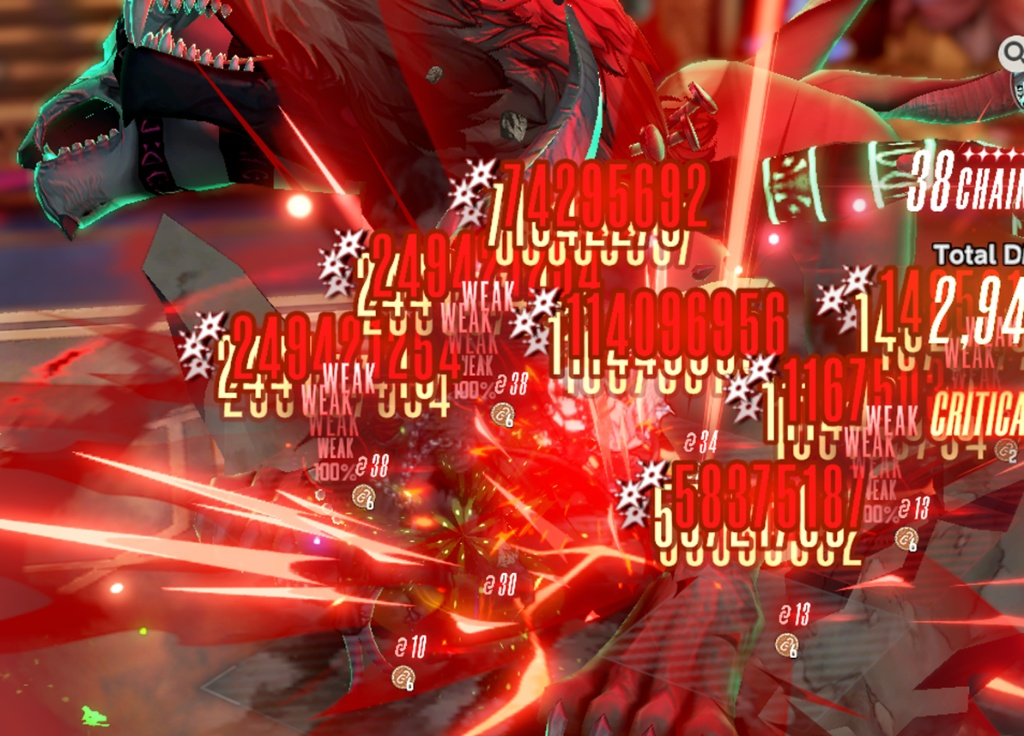
\includegraphics[width=0.75\textwidth]{figures/fiend-hunter-telemetry.jpg}
\caption{Live combat telemetry capture during AoE skillset execution on the Fiend Hunter boss. The floating damage numerals corroborate the simultaneous evaluations compiled in Table~\ref{tab:multitile_validation}.}
\label{fig:telemetry_multihit}
\end{figure}

As shown across all four impact nodes, the residual discrepancy between theoretical synthesis ($D_{\text{model}}$) and observable combat output ($D_{\text{observed}}$) scales strictly on the order of $\approx 10^{-6}\%$. We note that these four data points originate from a single AoE skillset execution frame and therefore share identical upstream base attributes, stochastic rolls, and persistent buff pools. Rather than an independent statistical regression, this multi-node cross-validation specifically confirms that local spatial variables ($\gamma_{\text{weak}}$ and $N_{\text{chain}}$) scale across simultaneous target tiles without introducing compounding numerical instability. The minor drift ($\Delta D \le 16$ across an amplitude exceeding $2.49 \times 10^8$) remains mathematically consistent with standard IEEE~754 single-precision mantissa rounding within the host engine.

\subsection{Scenario 2: Environmental Pressure Attenuation}

To isolate the operational boundaries of the Modifier Transformation Operator $\hat{\mathcal{T}}$, combat telemetry was evaluated across concurrent Critical Damage reinforcement channels alongside excess Critical Rate overflow under an active $70\%$ Environmental Pressure penalty ($P = 0.30$).

\subsubsection{Empirical Verification: Critical Multipliers and Overflow Invariance}

Unlike discrete integer attributes (ATK/MATK), which undergo channel-level truncation, percentage-denominated attributes remain continuous floating-point values throughout active status aggregation. Telemetry across multiple concurrent critical buffs confirms two structural engine behaviors:
\begin{itemize}
    \item \textbf{Linear Multi-Channel Scaling:} Concurrent external critical reinforcement channels ($\sum_j \vec{b}_j^{(\text{cdmg})}$) attenuate linearly by the pressure scalar $P = 0.30$ without inter-channel boundary drift.
    \item \textbf{Overflow Exemption:} Surplus Critical Rate ($\Delta \text{CR} = \max(0, \; \text{CR}_{\text{eff}} - 1.0)$) converts directly into $\Delta \text{CDMG}_{\text{ovf}}$ at nominal $100\%$ efficiency ($P = 1.0$), bypassing environmental status attenuation entirely.
\end{itemize}

As shown in Table~\ref{tab:cdmg_pressure_verification}, compounding multiple external CDMG reinforcement sources with excess rate conversion evaluates to the exact live combat hit with zero residual drift ($\Delta D = 0, R^2 = 1.0$).

\begin{table}[H]
\centering
\small
\setlength{\tabcolsep}{5pt}
\begin{tabular}{llr}
\toprule
\textbf{Channel / Operational Step} & \textbf{Component Parameter} & \textbf{Evaluated Value} \\
\midrule
\textbf{Native Base Stat}       & Pre-Combat Base CDMG ($v^{(\text{cdmg})}$)             & 516.12\% \\
\textbf{Reinforcement Pool}     & Cumulative CDMG Buffs ($\sum_j b_j^{(\text{cdmg})}$)    & 900\% \\
\textbf{Environmental Penalty}  & Pressure Scalar ($P = 1.0 - 0.70$)                    & $0.30$ \\
\textbf{Attenuated Buff Pool}   & $b_{\text{eff}} = \left(\sum_j b_j^{(\text{cdmg})}\right) \cdot P$ & 270\% \\
\midrule
\textbf{Native Base Stat}       & Pre-Combat Base Crit Rate ($v^{(\text{cr})}$)             & 68.80\% \\
\textbf{Reinforcement Pool}     & Cumulative Crit Rate Buffs ($\sum_j b_j^{(\text{cr})}$)    & 180\% \\
\textbf{Environmental Penalty}  & Pressure Scalar ($P = 1.0 - 0.70$)                    & $0.30$ \\
\textbf{Attenuated Buff Pool}   & $b_{\text{eff}} = \left(\sum_j b_j^{(\text{cr})}\right) \cdot P$ & 54\% \\
\textbf{Effective Crit Rate}    & Total Combat Crit Rate ($\text{CR}_{\text{eff}}$)             & 122.8\% \\
\textbf{Rate Surplus}           & $\Delta \text{CR} = \max(0, \; \text{CR}_{\text{eff}} - 1.0)$ & 22.8\% \\
\textbf{Overflow Conversion}    & $\Delta \text{CDMG}_{\text{ovf}} = \kappa_{\text{conv}} \cdot \Delta \text{CR} \quad (P = 1.0)$ & 136.8\% \\
\midrule
\textbf{Theoretical Composite Stat} & $\text{CDMG}_{\text{model}}$ ($= v^{(\text{cdmg})} + b_{\text{eff}} + \Delta \text{CDMG}_{\text{ovf}}$) & \textbf{922.92\%} \\
\textbf{Live Telemetry Stat}    & $\text{CDMG}_{\text{observed}}$     & \textbf{922.92\%} \\
\midrule\midrule
\textbf{Residual Drift}         & $\Delta D = CDMG_{\text{model}} - CDMG_{\text{observed}}$    & $\mathbf{0 \quad (R^2 = 1.0)}$ \\
\bottomrule
\end{tabular}
\caption{Empirical verification of multi-source Critical Damage attenuation and unscaled rate overflow under $70\%$ Environmental Pressure ($P = 0.30$).}
\label{tab:cdmg_pressure_verification}
\end{table}

\subsubsection{High-Density Buff Telemetry and Aggregator Decoupling}
When scaling to extreme buff density ($\ge 6$ concurrent reinforcement channels totaling $>800\%$ pre-pressure), an operational nuance emerges within the engine's pre-combat stat aggregator.

\begin{table}[H]
\centering
\small
\setlength{\tabcolsep}{6pt}
\begin{tabular}{lccc}
\toprule
\textbf{Metric / Pipeline Stage} & \textbf{Theoretical Model} & \textbf{In-Engine Telemetry} & \textbf{Residual Drift} \\
\midrule
Pre-Combat Base Stat ($v_1$)            & $1,708$            & $1,708$            & $0$ \\
Nominal Buff Scale ($\sum b_1 \cdot P$) & $+246.0\%$         & $+246.0\%$ (Input) & --- \\
\textbf{Added Stat Payload ($\Delta v_1$)} & $\mathbf{+4,201}$ & $\mathbf{+4,210}$ & $\mathbf{-9}$ \\
\textbf{Active Stat Vector ($v_{1,\text{active}}$)} & $\mathbf{5,909}$ & $\mathbf{5,918}$ & $\mathbf{-9}$ \\
\midrule
\multicolumn{4}{l}{\textit{Combat Kernel Execution (using In-Game Active Stat)}} \\
Discrete Base Payload ($M_{\text{base}}$) & $2603$ & 2603 & 0 \\
Terminal Damage Output ($D$)             & \textbf{4479} & \textbf{4479} & $\mathbf{\Delta D = 0}$ \\
\bottomrule
\end{tabular}
\caption{Decoupling of pre-combat stat compilation and combat kernel resolution under high-density environmental pressure ($P = 0.30$).}
\label{tab:pressure_high_density}
\end{table}

\paragraph{Empirical Decoupling: Stat Aggregator vs. Combat Kernel.}
The observed delta ($\Delta \text{ATK} \approx -9$) under high-density stacking does not reflect an error within the downstream combat equation. As demonstrated in Table~\ref{tab:pressure_high_density}, initializing the combat resolver with the engine's actual displayed active stat evaluates to the exact live damage payload with zero residual drift ($\Delta D = 0$). 

This cleanly isolates the $-9$ variance to the internal compilation phase of the entity's status effect manager under fractional pressure. While candidate mechanisms include internal accumulator rounding or truncation hysteresis across concurrent status instances, the downstream execution kernel is completely decoupled from this upstream aggregation variance.

\subsection{Scenario 3: Archetype Projection and Mitigation Bypass}

To validate the Coupling Factor $\gamma_{\text{def}}$ defined in Section~\ref{sec:damage_type_introduction}, combat telemetry was recorded using a Fixed Damage skill instance ($\gamma_{\text{def}} = 0, \; \gamma_{\text{barrier}} = 0$) against an active target possessing significant residual kinetic mitigations ($\text{DEF} / \text{MRES} > 0$).

Under the canonical mitigation bracket:
\begin{equation}
 M_{\text{res}} = \min \Big( 1, \; \max \left( 0.1, \; 1 - \gamma_{\text{def}} \cdot R_{\text{tgt}} \right) \Big)
\end{equation}

For standard kinetic attacks ($\gamma_{\text{def}} = 1, \; \gamma_{\text{barrier}} = 1$), non-zero defense and active barrier shields compound to severely attenuate incoming damage. On a target possessing $50\%$ DEF and an active $50\%$ Barrier, an unpenetrated kinetic strike would yield:
\begin{equation}
D_{\text{kinetic}} = \left\lfloor M_{\text{base}} \cdot (1 - 0.50) \cdot (1 - 0.50) \right\rfloor = \lfloor 1830 \times 0.25 \rfloor = 457
\end{equation}
Under fixed archetype projection ($\gamma_{\text{def}} = 0, \; \gamma_{\text{barrier}} = 0$), both mitigation gates collapse simultaneously to unity ($M_{\text{res}} \equiv 1.0, \; M_{\text{barrier}} \equiv 1.0$). 

As detailed in Table~\ref{tab:archetype_fixed_verification}, the live execution hit registers at exactly $D_{\text{observed}} = 1830$ ($\Delta D = 0$), confirming that incoming Fixed damage applies directly to target vitality without suffering the $75\%$ composite attenuation of the target's active defenses.

\begin{table}[H]
\centering
\small
\setlength{\tabcolsep}{5pt}
\begin{tabular}{llr}
\toprule
\textbf{Channel / Operational Step} & \textbf{Component Parameter} & \textbf{Evaluated Value} \\
\midrule
\textbf{Active Stat Vector}     & Attacker Effective Stat ($v_{1,\text{active}}$)    & 1220 \\
\textbf{Skill Multiplier}       & Fixed Skill Coefficient ($m_1$)                     & 150\% \\
\textbf{Discrete Base Payload}  & $M_{\text{base}} = \lfloor v_{1,\text{active}} \cdot m_1 \rfloor$ & 1830 \\
\midrule
\textbf{Target Kinetic Armor}   & Target Defense ($\text{DEF}$)               & 50\% \\
\textbf{Archetype Gate}         & Defensive Coupling Factor ($\gamma_{\text{def}}$) & $0.0$ \\
\textbf{Mitigation Multiplier}  & $M_{\text{res}} = 1.0 - \gamma_{\text{def}} \cdot \text{DEF}$ & $\mathbf{1.0000}$ \\
\midrule
\textbf{Target Barrier Status}  & Barrier Value ($r_{\text{j}}$)       & 50\% \\
\textbf{Archetype Gate}         & Barrier Coupling Factor ($\gamma_{\text{barrier}}$) & $0.0$ \\
\textbf{Barrier Multiplier}           & $M_{\text{barrier}} = 1.0 - \gamma_{\text{barrier}}\cdot r_j$ & $\mathbf{1.0000}$ \\
\midrule
\textbf{Combat Multipliers}     & $M_{\text{crit}} \cdot M_{\text{prop}} \cdot M_{\text{chain}} \dots$ & 1 \\
\midrule\midrule
\textbf{Theoretical Output}     & $D_{\text{model}} = \lfloor M_{\text{base}} \cdot \prod M_j \rfloor$ & \textbf{1830} \\
\textbf{Live Telemetry}         & $D_{\text{observed}}$ (Recorded Hit)               & \textbf{1830} \\
\midrule
\textbf{Residual Drift}         & $\Delta D = D_{\text{model}} - D_{\text{observed}}$ & $\mathbf{0 \quad (R^2 = 1.0)}$ \\
\bottomrule
\end{tabular}
\caption{Empirical verification of Fixed Damage archetype projection ($\gamma_{\text{def}} = 0, \gamma_{\text{barrier}} = 0$) bypassing kinetic mitigations and barrier absorption.}
\label{tab:archetype_fixed_verification}
\end{table}

% =========================================================================
% SECTION V: DISCUSSION AND CONCLUSION
% =========================================================================
\clearpage
\section{Discussion and Concluding Remarks}
\label{sec:conclusion}

This study established a phenomenological, closed-form mathematical framework that unifies the non-linear combat mechanics of the \textit{Brown Dust II} engine. By projecting entity interactions onto an orthogonal eight-dimensional state space ($\mathbb{R}^8$) and parameterizing conditional mechanics via binary archetype coupling factors ($\gamma_{\text{def}}, \gamma_{\text{barrier}}, \gamma_{\text{crit}}, \gamma_{\text{vuln}}$), the model encapsulates disparate runtime branching into a declarative algebraic pipeline while preserving analytical tractability.

\subsection{Architectural Synthesis}
Empirical verification across diverse live-server telemetry environments confirmed three primary architectural principles governing the execution pipeline:
\begin{enumerate}
    \item \textbf{Aggregator--Kernel Decoupling:} The host engine maintains a strict structural boundary between pre-combat entity state compilation and downstream combat resolution. While macro-progression and status effect instances undergo intermediate integer truncation within the entity stat aggregator, the downstream combat kernel executes across continuous floating-point registers, culminating in a single discrete floor operation at terminal synthesis (yielding exact telemetry convergence, $\Delta D = 0$).
    \item \textbf{Environmental Attenuation Boundaries:} Environmental Pressure ($P$) operates selectively on positive reinforcement status pools ($\vec{b}_j$), exhibiting total invariance across downstream conversion mechanics—most notably surplus Critical Rate overflow ($\Delta \text{CDMG}_{\text{ovf}}$), which transfers into the terminal critical multiplier at nominal $100\%$ efficiency.
    \item \textbf{Mitigation Projection Collapse:} Fixed and Pure damage archetypes successfully collapse both kinetic armor brackets ($M_{\text{res}} \equiv 1.0$) and multiplicative barrier cascades ($M_{\text{red}} \equiv 1.0$) simultaneously, validating the declarative binary gate identity $\gamma_{\text{barrier}} \equiv \gamma_{\text{def}}$.
\end{enumerate}

\subsection{Implications for Team Optimization}
The formalized Master Equation (Eq.~\ref{eq:master_monolithic}) provides actionable constraints for automated team sequencing algorithms:
\begin{itemize}
    \item \textbf{Marginal Modifier Yields:} Because external offensive amplifications ($M_{\text{base}}, M_{\text{prop}}, M_{\text{chain}}, M_{\text{vuln}}$) compound multiplicatively while intra-channel modifiers aggregate additively, optimal turn sequences prioritize distributing buff categories across orthogonal brackets rather than over-saturating a single status pool.
    \item \textbf{Surplus Conversion Thresholds:} The linear $1:6$ Critical Rate overflow ratio ($\kappa_{\text{conv}} = 6.0$) provides a quantifiable inflection point: once Critical Rate reaches saturation ($1.0$), excess rate investment provides superior marginal scaling compared to direct additive CDMG gear rolls whenever base CDMG exceeds nominal equipment caps.
\end{itemize}

\subsection{Limitations and Future Work}
While the downstream damage kernel achieves near-zero error ($\text{MAPE} < 7 \times 10^{-6}\%$ across high-amplitude nukes), the upstream pre-combat aggregator exhibits minor integer drift ($\Delta \text{ATK} \le 9$) under extreme buff stacking ($\ge 6$ concurrent sources) within fractional pressure environments. Future research will focus on decompiling the entity status manager's internal loop to determine whether this variance stems from intermediate accumulator rounding, truncation hysteresis, or order-dependent channel registration.

\begin{thebibliography}{9}

\bibitem{ieee754}
IEEE Computer Society,
\textit{IEEE Standard for Floating-Point Arithmetic},
IEEE Std 754-2019, pp.~1--84, 2019.

\bibitem{sequencer}
Souseha,
\textit{Brown Dust 2 Formation Templates Archive},
Interactive combat log repository, 2026. [Online]. Available: \url{https://browndust2-db.souseha.com/en/formation/preview?id=8qtDcpvoHFzoD0XjP1xR}

\end{thebibliography}


\renewcommand{\refname}{Data and Telemetry Sources}
\begin{thebibliography}{9}
\bibitem{gamereference}
GAMFS N,
\textit{Brown Dust II Game Client Execution Environment},
Unity Engine / C\# Combat Pipeline, Live Server Build Version~2.33.15, Neowiz, 2026.
\end{thebibliography}

\end{document}